\subsection{RS-Flipflop} % (fold)
\label{sub:RS-Flipflop}
\begin{frame}
    \frametitle{RS-Flipflop}
    \framesubtitle{}
    \begin{figure}[H]
    \begin{center}
            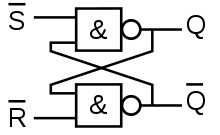
\includegraphics[scale=0.5]{./img/schaltung/RS-FF.png}
    \end{center}
    \end{figure}
\end{frame}
\begin{frame}
    \frametitle{Funktionsweise}
    \framesubtitle{}
    \begin{columns}[c]
        \column{0.6\textwidth}
            \boxed{
                \begin{tabular}{c|c||c}
                    $\bar{S}$ & $\bar{R}$ & Q \\
                    \hline
                    1 & 1 & unverändert \\
                    0 & 1 & 1 (gesetzt) \\
                    1 & 0 & 0 (zurückgesetzt) \\
                    0 & 0 & Glitch ($Q = \bar{Q}$)
                \end{tabular}
                }
            \begin{block}{Gleizeitiges Auslößen}
                \begin{itemize}
                    \item Beide Lampen leuchten auf 
                \end{itemize}
            \end{block}
        \column{0.4\textwidth}
            \begin{figure}[H]
            \begin{center}
                    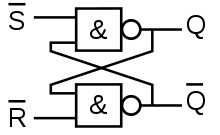
\includegraphics[scale=0.5]{./img/schaltung/RS-FF.png}
            \end{center}
            \end{figure}
    \end{columns}
\end{frame}
% subsection RS-Flipflop (end)
